
%(BEGIN_QUESTION)
% Copyright 2007, Tony R. Kuphaldt, released under the Creative Commons Attribution License (v 1.0)
% This means you may do almost anything with this work of mine, so long as you give me proper credit

Tegn responsen til en regulator med proporsjonal + integralvirkning for følgende inngangsbetingelser, med antatt proporsjonalbånd på 100\% og integralkonstant 8 minutter per repetisjon. Regulatoren er {\it direktevirkende}, og algoritmen den følger er vist under grafen:

$$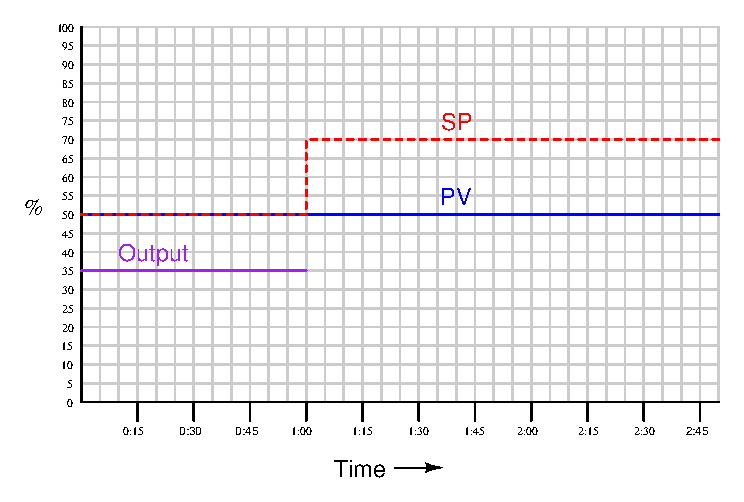
\includegraphics[width=15.5cm]{i01603x01.eps}$$

Tidsskalaen i diagrammet er minutter:sekunder, og PI-algoritmen er som følger:

$$m = K_p \left( e + {1 \over \tau_i} \int e \> dt \right) + b$$

\noindent
Der,

$m$ = regulatorutgang (manipulert variabel)

$K_p$ = forsterkning

$e$ = avvikssignal (PV$-$SP)

$\tau_i$ = integraltidskonstant

$b$ = bias

\vskip 10pt

\underbar{file i01603}
%(END_QUESTION)





%(BEGIN_ANSWER)

$$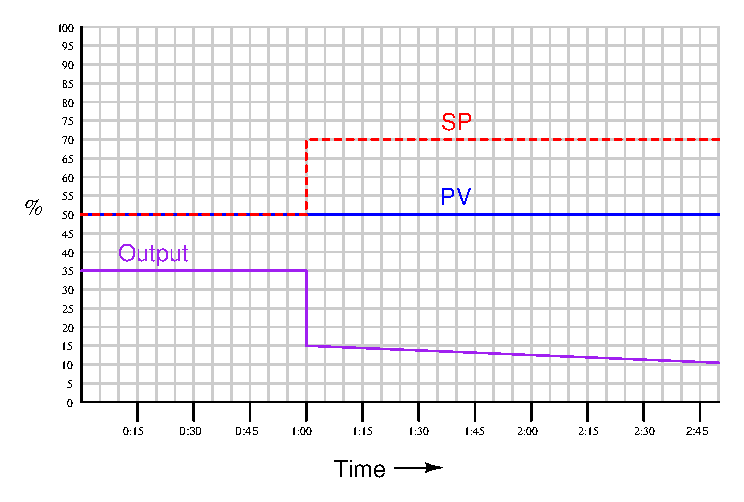
\includegraphics[width=15.5cm]{i01603x02.eps}$$

%(END_ANSWER)





%(BEGIN_NOTES)

En integralkonstant på 8 minutter per repetisjon (0.125 repetisjoner per minutt) gjør at utgangskurven får en relativt svak (flat) stigning. Den akkumulerer en utgangsendring på 2.5\% på 1 minutt.

%INDEX% Control, proportional + integral: graphing controller response

%(END_NOTES)
